\documentclass{article}
\usepackage{amsfonts,amssymb,amsmath,amsthm}

%% set-style letters
\def\AA{{\mathbb{A}}}
\def\BB{{\mathbb{B}}}
\def\CC{{\mathbb{C}}}
\def\DD{{\mathbb{D}}}
\def\EE{{\mathbb{E}}}
\def\FF{{\mathbb{F}}}
\def\GG{{\mathbb{G}}}
\def\HH{{\mathbb{H}}}
\def\II{{\mathbb{I}}}
\def\JJ{{\mathbb{J}}}
\def\KK{{\mathbb{K}}}
\def\LL{{\mathbb{L}}}
\def\MM{{\mathbb{M}}}
\def\NN{{\mathbb{N}}}
\def\OO{{\mathbb{O}}}
\def\PP{{\mathbb{P}}}
\def\QQ{{\mathbb{Q}}}
\def\RR{{\mathbb{R}}}
\def\SS{{\mathbb{S}}}
\def\TT{{\mathbb{T}}}
\def\UU{{\mathbb{U}}}
\def\VV{{\mathbb{V}}}
\def\WW{{\mathbb{W}}}
\def\XX{{\mathbb{X}}}
\def\YY{{\mathbb{Y}}}
\def\ZZ{{\mathbb{Z}}}

%% calligraphic letters
\def\cA{{\mathcal{A}}}
\def\cB{{\mathcal{B}}}
\def\cC{{\mathcal{C}}}
\def\cD{{\mathcal{D}}}
\def\cE{{\mathcal{E}}}
\def\cF{{\mathcal{F}}}
\def\cG{{\mathcal{G}}}
\def\cH{{\mathcal{H}}}
\def\cI{{\mathcal{I}}}
\def\cJ{{\mathcal{J}}}
\def\cK{{\mathcal{K}}}
\def\cL{{\mathcal{L}}}
\def\cM{{\mathcal{M}}}
\def\cN{{\mathcal{N}}}
\def\cO{{\mathcal{O}}}
\def\cP{{\mathcal{P}}}
\def\cQ{{\mathcal{Q}}}
\def\cR{{\mathcal{R}}}
\def\cS{{\mathcal{S}}}
\def\cT{{\mathcal{T}}}
\def\cU{{\mathcal{U}}}
\def\cV{{\mathcal{V}}}
\def\cW{{\mathcal{W}}}
\def\cX{{\mathcal{X}}}
\def\cY{{\mathcal{Y}}}
\def\cZ{{\mathcal{Z}}}
\def\cKL{{\mathcal{KL}}}

%% bold letters
\def\bA{{\bf{A}}}
\def\bB{{\bf{B}}}
\def\bC{{\bf{C}}}
\def\bD{{\bf{D}}}
\def\bE{{\bf{E}}}
\def\bF{{\bf{F}}}
\def\bG{{\bf{G}}}
\def\bH{{\bf{H}}}
\def\bI{{\bf{I}}}
\def\bJ{{\bf{J}}}
\def\bK{{\bf{K}}}
\def\bL{{\bf{L}}}
\def\bM{{\bf{M}}}
\def\bN{{\bf{N}}}
\def\bO{{\bf{O}}}
\def\bP{{\bf{P}}}
\def\bQ{{\bf{Q}}}
\def\bR{{\bf{R}}}
\def\bS{{\bf{S}}}
\def\bT{{\bf{T}}}
\def\bU{{\bf{U}}}
\def\bV{{\bf{V}}}
\def\bW{{\bf{W}}}
\def\bX{{\bf{X}}}
\def\bY{{\bf{Y}}}
\def\bZ{{\bf{Z}}}
\def\ba{{\bf{a}}}
\def\bb{{\bf{b}}}
\def\bc{{\bf{c}}}
\def\bd{{\bf{d}}}
\def\be{{\bf{e}}}
\def\boldf{{\bf{f}}} %different
\def\bg{{\bf{g}}}
\def\bh{{\bf{h}}}
\def\bi{{\bf{i}}}
\def\bj{{\bf{j}}}
\def\bk{{\bf{k}}}
\def\bl{{\bf{l}}}
\def\bm{{\bf{m}}}
\def\bn{{\bf{n}}}
\def\bo{{\bf{o}}}
\def\bp{{\bf{p}}}
\def\bq{{\bf{q}}}
\def\br{{\bf{r}}}
\def\bs{{\bf{s}}}
\def\bt{{\bf{t}}}
\def\bu{{\bf{u}}}
\def\bv{{\bf{v}}}
\def\bw{{\bf{w}}}
\def\bx{{\bf{x}}}
\def\by{{\bf{y}}}
\def\bz{{\bf{z}}}

%% other symbols
\DeclareMathOperator{\1}{\mathbf{1}}
\DeclareMathOperator{\0}{\mathbf{0}}
\DeclareMathOperator{\Id}{I}
\newcommand{\td}{\mathfrak{t}} % discrete-time 
\newcommand{\tr}{^\top}

%% operators
\DeclareMathOperator{\col}{col}
\DeclareMathOperator{\diag}{diag}
\DeclareMathOperator{\blkdiag}{blkdiag}
\DeclareMathOperator{\rank}{rank}
\DeclareMathOperator{\dis}{d}
\DeclareMathOperator{\sat}{sat} 
\DeclareMathOperator{\convhull}{\textbf{co}}
\DeclareMathOperator{\argmin}{argmin}
\DeclareMathOperator{\argmax}{argmax}
\DeclareMathOperator{\spec}{spec}
\def\He#1{\texttt{\rm{He}}\left\{{#1}\right\}}
\DeclareMathOperator{\trace}{tr}
\newcommand{\Imag}{\mathrm{Im}}

%% shortcuts
\newcommand{\norm}[1]{\lvert #1\rvert}
\newcommand{\wnorm}[2]{\lvert #1\rvert^2_{#2}}
\newcommand{\pderiv}[2]{\dfrac{\partial #1}{\partial #2}}
\newcommand{\pdef}[1]{\SS_{\succ0}^{#1}}
\newcommand\psemidef[1]{\SS_{\succeq0}^{#1}}
\newcommand{\bmx}[1]{\left[\begin{matrix}#1\end{matrix}\right]}
\newcommand{\pmx}[1]{\left(\begin{matrix}#1\end{matrix}\right)}
\newcommand{\smallpmat}[1]{\left(\begin{smallmatrix} #1 \end{smallmatrix} \right)}
\newcommand{\smallqmat}[1]{\left[\begin{smallmatrix} #1 \end{smallmatrix} \right]}
\newcommand{\overbar}[1]{\mkern 1.5mu\overline{\mkern-1.5mu#1\mkern-1.5mu}\mkern 1.5mu}
\renewcommand{\underbar}[1]{\mkern 1mu\underline{\mkern-1mu#1\mkern-1mu}\mkern 1mu}

\usepackage{hyperref}
\usepackage{graphicx}
\usepackage{float}

% SCRIPTS FOR DOUBLE AND SINGLE IMAGE

% \begin{figure}[H]
%     \centering
%     \begin{subfigure}{0.4\textwidth}
%     \includegraphics[width=\textwidth]{}
%     \caption{}
%     \label{}
%     \end{subfigure}
%     \hfill
%     \begin{subfigure}{0.55\textwidth}
%     \includegraphics[width=\textwidth]{}
%     \caption{}
%     \label{}
%     \end{subfigure}
%     \caption{}
%     \label{}
% \end{figure}

% \begin{figure}[H]
%     \centering
%     \includegraphics[width=0.65\textwidth]{}
%     \caption{}
%     \label{}
% \end{figure}

\usepackage{biblatex}
\addbibresource{../biblio.bib}

\begin{document}

\title{Draft of paper}

\author{Marco Sterlini}


\section{Introduction}

\section{Problem Formulation}
We consider the non-linear discrete-time system stabilized by a Neural Network (NN) controller represented in figure \ref{fig:first_scheme} described by:
\begin{equation}
  x^{+} = A x + B \texttt{sat}(\bar{u}) + C \Phi(E x) + D d 
\end{equation}
where the saturation function \texttt{sat} is defined as:
$$
    \texttt{sat}(\bar{u}) = \texttt{sign}(\bar{u})\text{min}(|\bar{u}|, \hat{u})
$$
with $\hat{u}$ the lmit of the input signal, $x \in \RR^{n_x}$ the state vector, $\bar{u} \in \RR^{n_u}$ the raw output of the controller, $\Phi \in \RR^{n_q}$ the representation of the non-linearity of the system \textbf{ADD MORE DETAILS ABOUT THE NON-LINEARITY SINCE ITS NOLCOS} and $d \in \RR^{n_d}$ a constant disturbance input.

\begin{figure}[H]
    \centering
    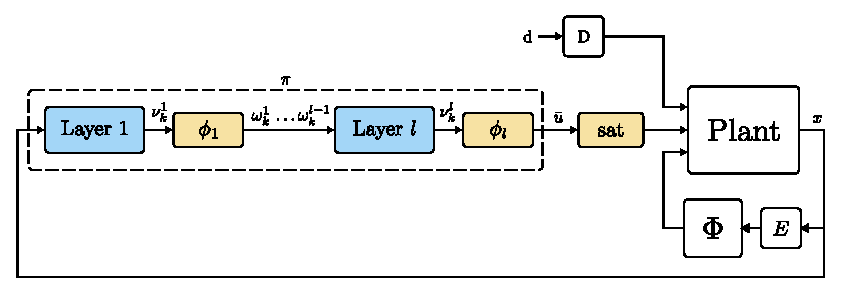
\includegraphics[width=0.45\textwidth]{Figures/first_scheme}
    \caption{Feedback system}
    \label{fig:first_scheme}
\end{figure}

The controller is implemented as a Multi Layer Perceptron (MLP) with $l$ layers, each with $n_{\phi_i}, i \in \left\{ 1, \dots, l\right\}$ neurons, all activation functions are saturation functions, represented by $\phi_i$. The objective is to design an Event-Triggering Mechanism (ETM) that allows to ease the computational burden associated with the computation of many non-linear activation functions providing at the same time sufficient sector conditions to handle the non-linearity of the system and the controller. The controller $\pi$ is defined by:
\begin{equation}\label{eq:nn-equations}
  \begin{aligned}
  \omega^{0}(k) &= x(k) \\
  \nu^{i}(k) &= W^{i} \omega^{i - 1}(k) + b^{i}, i \in \left\{ 1, \dots, l \right\}\\
  \omega^{i}(k) &= \phi_i(\nu^i(k))\\
  \bar{u}(k) &= \phi_l(\nu^l(k))
  \end{aligned} 
\end{equation}
with $\nu^i(k) \in \RR^{n_{\phi_i}}$ the input to the $i$-th activation function $\phi_i: \RR^{n_{\phi_i}} \to \RR^{n_{\phi_i}}$, $\omega^i(k) \in \RR^{n_{\phi_i}}$ the output. The weights $W^i \in \RR^{n_{\phi_i} \times n_{\phi_{i-1}}}$ and biases $b^i \in \RR^{n_{\phi_i}}$ define the affine operation of each layer. The saturation function application is to be intended element-wise and will be denoted as $\phi_i(\nu^i(k)) = \left[ \varphi(\nu^i_1(k)), \dots, \varphi(\nu^i_{n_{\phi_i}}(k)) \right]$ and $\varphi: \RR \to \RR$ is the scalar activation function assumed to be symmetric and identical for every neuron. Adopting the same notation as in \cite{css-paper} we define the controller policy in a condensed form. Denoting the augmented vectors:
\begin{equation*}
  \nu = \bmx{\nu^1 \\ \vdots \\ \nu^l}, \omega = \bmx{\omega^1 \\ \vdots \\ \omega^l}, \phi = \bmx{\phi_1(\nu^1) \\ \vdots \\ \phi_l(\nu^l)} 
\end{equation*}
with $n_{\phi} = \sum_{i=1}^{l} n_{\phi_i}$ and $\phi: \RR^{n_{\phi}} \to \RR^{n_{\phi}}$ the combined non-linearity we have $\omega = \phi(\nu)$. Finally, conditions \ref{eq:nn-equations} can be rewritten as:
\begin{equation*}
  \bmx{u(k)\\ \nu(k)} = N \bmx{x(k) \\ \omega(k) \\ 1} 
\end{equation*}
where
\begin{equation}\label{eq:first-N}
  \bmx{
    \begin{array}{c | c c c c | c}
      \0 & \0 & \dots & \0 & W^l & b^l \\ 
      \hline
      W^1 & \0 & \dots & \0 & \0 & b^1 \\
      \0 & W^2 & \dots & \0 & \0 & b^2 \\
      \vdots & \vdots & \ddots & \vdots & \vdots & \vdots \\
      \0 & \0 & \dots & W^{l-1} & \0 & b^{l-1}
    \end{array}
  }
\end{equation}
Similarly as in \cite{css-extended} we implement an ETM in every layer of the controller, we add also a final one to the output that will be used to further reduce the total number of events and calls to the non-linear functions. The system and the controller are now described by figure \ref{fig:second_scheme}.
\begin{figure}[H]
    \centering
    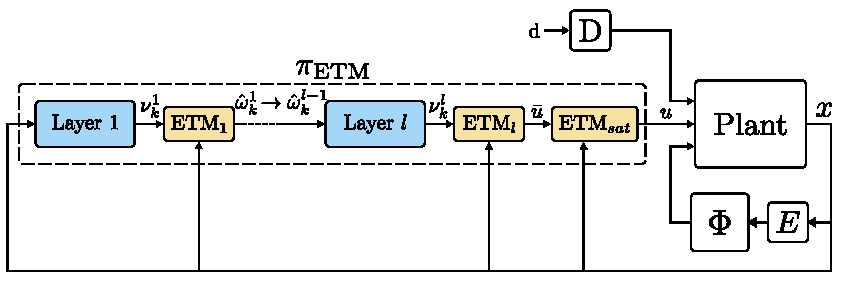
\includegraphics[width=0.45\textwidth]{Figures/second_scheme}
    \centering
    \caption{Feedback system subject to ETM in the controller}
    \label{fig:second_scheme}
\end{figure}
The dynamics will be rewritten as:
\begin{equation}\label{eq:system-dynamics}
  x^{+} = A x + B u + C \Phi(E x) + D d
\end{equation}
with $u \in \RR^{n_u}$ the output of the controller subject to the ETM. This modification required to redefine the matrix $N$ defined in the controller policy \ref{eq:first-N} as:
\begin{equation}\label{eq:last-N}
  N = \bmx{
    \begin{array}{c | c c c c | c}
      \0 & \0 & \dots & \0 & \Id & 0 \\ 
      \hline
      W^1 & \0 & \dots & \0 & \0 & b^1 \\
      \0 & W^2 & \dots & \0 & \0 & b^2 \\
      \vdots & \vdots & \ddots & \vdots & \vdots & \vdots \\
      \0 & \0 & \dots & W^l & \0 & b^l
    \end{array}
  } = \bmx{
    \begin{array}{c | c | c}
    N_{u x} & N_{u \omega} & N_{u b} \\
    \hline
    N_{\nu x} & N_{\nu \omega} & N_{\nu b}
    \end{array} 
  }
\end{equation}
All the non-linearity of the system and the controller are selected as saturation functions. With respect to \cite{css-extended}, Lemma 3, we declare the local sector conditions that hold for this function:

\emph{For $i \in \left\{ 1, \dots, l \right\}$ given a matrix $G^i \in \RR^{n_{\phi_i} \times n_x}$, if $x(k)$ belongs to the set}
$$
S^i = \left\{ x(k) \in \RR^{n_x} : -\bar{\nu}^i - \bar{\nu}_* \leq G^i (x(k) - x_*) \leq \bar{\nu}^i - \nu_*^i \right\} 
$$

\emph{Then the following quadratic constraint holds for any diagonal positive definite matrix $T^i \in \RR^{n_{\phi_i} \times n_{\phi_i}}$:}
\begin{equation}\label{eqn:first_sec_cond}
  \left[ \nu^i(k) - \omega^i(k) \right]\tr T^i \left[ G^i (x(k) - x_*) - (\omega^i(k) - \omega^i_*) \right] \leq 0
\end{equation}

The system is compliant with the assumptions of \textbf{Lemma 2} in \cite{css-extended} that allow us to define the following expressions regarding the equilibrium points $\left( x_*, u_*, \nu_*, \omega_* \right)$ of the system and controller given $x_*$, defining the matrices:
\begin{equation}
    \begin{aligned}
         R &= (\Id - N_{\nu \omega})^{-1}\\
         R_{\omega} &= N_{u x} + N_{u \omega} R N_{\nu x}\\
         R_b &= N_{u \omega} R N_{\nu b} + N_{u b}
    \end{aligned}
\end{equation}

With $N_{\nu \omega}$ always invertible due to its lower triangular structure. We find the equilibrium of the state by the use of a numerical solver that minimizes the following expression since it is no longer explicit due to the non-linearity $\Phi$. Given a constant disturbance $\bar{d}$:
\begin{equation}
  x_* = \min_{x} \left[(A + B R_{\omega} - \Id) x + C \Phi(E x) + D \bar{d} + B R_b \right]
\end{equation}
\begin{equation}\label{eqn:equilibrium}
  \bmx{u_* \\ \nu_*} = N \bmx{x_* \\ \omega_* \\ 1}; \ \  
  \begin{aligned}
    \omega_* &= \nu_*\\
    \nu_* &= R N_{\nu x} x_* + R N_{\nu b}\\
    u_* &= R_{\omega} x_* + R_b
  \end{aligned}
\end{equation}
In order to have a lighter notation the dead-zone vector  will be defined as $\psi = \nu - \omega$. Furthermore, all following discussions will take into account incremental variables with respect to their equilibrium, denoted with a tilde, i.e. $\tilde{x} = x - x_*$. Considering \ref{eqn:equilibrium} we have $\psi_* = \nu_* - \omega_* = 0$ hence $\tilde{\psi} = \psi$. The sector condition \ref{eqn:first_sec_cond} can be rewritten with no loss of generality as:
\begin{equation}\label{eqn:sec_cond}
  \tilde{\psi}\tr T^i \left[ G^i \tilde{x} + \tilde{\psi} - \tilde{\nu} \right] \leq 0
\end{equation}
We can express now the new inter-dependency between the variables of interest:
\begin{equation}\label{eqn:incremental}
  \begin{aligned}
    \tilde{u} &= R_{\omega} \tilde{x} - N_{u \omega} R \tilde{\psi}\\
    \tilde{\nu} &= R N_{\nu x} \tilde{x} + (\Id - R) \tilde{\psi}
  \end{aligned}
\end{equation}

\section{Main Results}
Taking inspiration from \textbf{Proposition 1} and \textbf{Lemma 3} in \cite{css-extended} we design the ETM for the output of each layer of the controller and the final output. The original idea was to trigger an event whenever the sector conditions were violated.

\subsection{Event-triggering mechanism}
An ETM works by triggering an event that will update the current layer and propagate its value across the network. The triggering function will take as inputs the incremental variables of the state of the system 
$\tilde{x}$, the current state of the layer $\tilde{\nu}$ and the dead-zone vector $\tilde{\psi}$. The ETM was defined as:
\begin{equation}
  \omega^{i}(k) = \begin{cases}
    \phi_i(\nu^i(k)) & \text{if } f^i(\tilde{x}, \tilde{\psi}, \tilde{\nu}) > 0\\
    \omega^{i}(k-1) & \text{otherwise}
  \end{cases}
\end{equation}
In the precedent work \cite{css-extended} the function $f$ is defined on the basis of the saturation sector conditions in the following quadratic form with respect to \ref{eqn:sec_cond}:
\begin{equation}\label{eqn:base_omega}
  f^i(\tilde{x}, \tilde{\psi}, \tilde{\nu}) =
  \bmx{\tilde{x}\\ \tilde{\psi} \\ \tilde{\nu}}\tr
  \Omega^i
  \bmx{\tilde{x}\\ \tilde{\psi} \\ \tilde{\nu}} > 0
\end{equation}
With $$
\Omega^i =  \bmx{
    0 & 0 & 0\\
    T^i G^i & T^i & -T^i\\
    0 & 0 & 0
  } 
$$

This approach acts as a static ETM triggering an event immediately after the sector conditions are violated. Inspired by the work of \cite{data-driven} we define a dynamic quantity to be implemented in the ETM triggering condition. The idea is to lower the conservatism of the controller by introducing a time-varying threshold that will adapt to the current state of the system reducing the overall number of events and computational burden. The new triggering function for the new \emph{dynamic-ETM} is defined as:
\begin{equation}\label{eqn:dynamic_trig}
  \omega^{i}(k) = \begin{cases}
    \phi_i(\nu^i(k)) & \text{if } f^i(\tilde{x}, \tilde{\psi}, \tilde{\nu}) > \rho^i \eta_i\\
    \omega^{i}(k-1) & \text{otherwise}
  \end{cases};
\end{equation}

Where $\eta^i$ characterized by the following dynamics:
\begin{equation}\label{eqn:eta_dynamics}
  \eta^+_i = \rho^i \eta_i - f^i(\tilde{x}, \tilde{\psi}, \tilde{\nu})\  \forall i \in \left( 1, \dots, l \right) 
\end{equation}

\textbf{Remark} \emph{Similarly as in Lemma 3 of \cite{data-driven} we will demonstrate how $\eta^i_k$ being the dynamic threshold of layer $i$ at time instant $k$ is non-negative for any $\rho^i \in [0, 1)$, $\eta^i_0 \geq\ \forall k \in \NN$}

\textbf{Proof} We consider the dynamics \ref{eqn:eta_dynamics} and the ETM triggering rule \ref{eqn:dynamic_trig} we prove the remark by recursion:\\
\emph{Initial condition}: Assuming $\eta^i_0 \geq 0$ we may have two possible outcomes:
if $f^i(\tilde{x}, \tilde{\psi}, \tilde{\nu}) < \rho^i \eta^i_0$ we have that 
\begin{equation}
  f^i(\tilde{x}, \tilde{\psi}, \tilde{\nu}) < \rho^i \eta^i_0 \to \rho^i \eta^i_0 - f^i(\tilde{x}, \tilde{\psi}, \tilde{\nu}) = \eta^i_1 \geq 0
\end{equation}

If instead $f^i(\tilde{x}, \tilde{\psi}, \tilde{\nu}) > \rho^i \eta^i_0$ then the event is triggered and the values of the current layer state $(\tilde{\psi}, \tilde{\nu})$ are updated to $(\bar{\psi}, \bar{\nu})$, leading again to the first case scenario where $f^i(\tilde{x}, \bar{\psi}, \bar{\nu}) < \rho^i \eta^i_0 \to \eta^i_1 \geq 0$.\\
\emph{Recursion step}: Assuming $\eta^i_k \geq 0$ similarly as the initial condition we may have:
$$
f^i(\tilde{x}, \tilde{\psi}, \tilde{\nu}) < \rho^i \eta^i_k \to \rho^i \eta^i_k - f^i(\tilde{x}, \tilde{\psi}, \tilde{\nu}) = \eta^i_{k+1} \geq 0
$$
If $f^i(\tilde{x}, \tilde{\psi}, \tilde{\nu}) > \rho^i \eta^i_k$ once again the event is triggered, we update $(\tilde{\psi}, \tilde{\nu}) \to (\bar{\psi}, \bar{\nu})$, the triggering function switches sign $f^i(\tilde{x}, \bar{\psi}, \bar{\nu}) < \rho^i \eta^i_k \to \eta^i_{k+1} \geq 0$.\\
Hence, $\eta^i_k \geq 0$ implies $\eta^i_{k+1} \geq 0$ concluding the recursion proof.


We denote a condensed notation by taking into account all conditions for each layer
\begin{equation}
\begin{aligned}
   \bR &= \text{diag} \pmx{\rho^1 & \dots & \rho^l }\\
   \mathbf{\Psi} &= \text{diag} \pmx{ f^1 & \dots & f^l }\\ 
   \boldsymbol{\eta} &= \text{diag} \pmx{ \eta^1 & \dots & \eta^l }   
\end{aligned}
\end{equation}

The ETM triggering condition and dynamic thresholds' dynamics can be rewritten in an element-wise fashion as:
\begin{equation}
\begin{aligned}
    \boldsymbol{\eta}^+ &= \bR \boldsymbol{\eta} - \mathbf{\Psi}\\
    \mathbf{\Psi} &> \bR \boldsymbol{\eta}
\end{aligned}
\end{equation}

\subsection{Finsler Lemma application}
After the implementation of the dynamic threshold a further improvement of the triggering condition has been taken in consideration. More precisely by denoting $\xi^i = (\tilde{x}, \tilde{\psi}^i, \tilde{\nu}^i)$ we rewrite the even triggering condition $f^i(\tilde{x}, \tilde{\psi}, \tilde{\nu}) > \rho^i \eta^i$ by taking in consideration \ref{eqn:base_omega} as 
\begin{equation}
    {\xi^i}\tr \Omega^i \xi^i > \rho^i \eta^i
\end{equation}
Intuitively the lower the left-hand term of the inequality the lower will be the number of triggered events. Unfortunately $\Omega^i$ structure is non-flexible due to his strict relation with the sector condition expression. The following lemma addresses the issue by designing some triggering matrices that guarantee a lower update rate for each layer by the use of Finsler's lemma:

\textbf{Lemma 1}: \emph{Considering the triggering policy \ref{eqn:dynamic_trig}, $R^i$ such that $\bmx{\tilde{x} & \tilde{\psi}^i & \tilde{\nu}^i}\tr = R^i \bmx{\tilde{x} & \tilde{\psi} & \tilde{\nu}}\tr \to {\xi^i}\tr = R^i \xi\tr$ and assuming \ref{eqn:incremental} holds $\forall \xi \in \left[ \underline{\xi}, \bar{\xi}\right]$, if $\exists X^i \in \RR^{nx + 2n_{\phi_i} \times nx + 2n_{\phi_i}}, N^i_1 \in \RR^{n_x \times n_{\phi_i}}, N^i_2, N^i_3 \in \RR^{n_{\phi_i} \times n_{\phi_i}}$ such that:
\begin{equation}\label{eqn:finsler}
     {R^i}\tr He\left\{X^i - \Omega^i\right\} R^i + He\left\{ \pmx{N^i_1\\ N^i_2\\ N^i_3} \pmx{R N_{\nu x} & \Id - R & -\Id}\right\} \leq 0
\end{equation}
Then we have ${\xi^i}\tr X^i \xi^i \leq {\xi^i}\tr \Omega^i \xi^i$}

\textbf{Proof} By pre and post multiplying for $\xi$ the previous expression we end up with
$$
    {\xi^i}\tr He\left\{X^i - \Omega^i\right\} \xi^i + He\left\{ \xi\tr \pmx{N^i_1\\ N^i_2\\ N^i_3} \pmx{R N_{\nu x} & \Id - R & -\Id} \xi \right\} \leq 0
$$
By expanding the term $\pmx{R N_{\nu x} & \Id - R & -\Id} \xi$ we end up with condition \ref{eqn:incremental} meaning that the expression is reduced to
$$
    {\xi^i}\tr He(X^i - \Omega^i) \xi^i \leq 0
$$
By further expanding the expression and considering that it is eventually reduced to a scalar for which it holds that the transpose is equivalent to itself we obtain:  
\begin{equation*}
\begin{aligned}
    &{\xi^i}\tr (X^i + {X^i}\tr) \xi^i \leq {\xi^i}\tr (\Omega^i + {\Omega^i}\tr) \xi^i\\
    &2 {\xi^i}\tr X^i\xi^ \leq 2 {\xi^i}\tr \Omega^i \xi^i\\
    & {\xi^i}\tr X^i \xi^i \leq {\xi^i}\tr \Omega^i \xi^i
\end{aligned}
\end{equation*}

Assuming we have the $X^i$ matrices $i \in \left\{1, \dots, l \right\}$ we rewrite the triggering conditions for each layer:
\begin{equation}
  \omega^{i}(k) = \begin{cases}
    \phi_i(\nu^i(k)) & \text{if } {\xi^i}\tr X^i \xi > \rho^i \eta^i(k)\\
    \omega^{i}(k-1) & \text{otherwise}
  \end{cases}
\end{equation}
By denoting $\bX = \text{diag} \pmx{{R^1}\tr X^1 R^1 & \dots & {R^l}\tr X^l R^l}$, the ETM triggering condition and dynamic thresholds' dynamics can be rewritten in an element-wise fashion as:
\begin{equation}
\begin{aligned}
    \boldsymbol{\eta}^+ &= \bR \boldsymbol{\eta} - \bX \\
    \bX &> \bR \boldsymbol{\eta}\end{aligned}
\end{equation}

\subsection{Lyapunov conditions}
In this section we will provide sufficient conditions for the stability of the system and the controller under the form of Linear Matrix Inequalities (LMIs) with the guarantee of local asymptotic stability. The solution of the problem will also provide the matrices $X^i$ and the parameters $\rho^i$ that will be used in the ETM triggering conditions along with an estimate of the Region Of Attraction (ROA) of the equilibrium point. 

We will first introduce a more compact notation for the system dynamics as long as some auxiliary matrices:
\begin{equation}
\begin{aligned}
    \bar{A} &= A + B R_{\omega}\\
    \bar{B} &= -B N_{u \omega} R\\
\end{aligned};\ \ 
R_{\nu} = \bmx{
  \Id & \0 & \0 & \0\\
  \0 & \Id & \0 & \0\\
  R N_{\nu x} & \Id - R & \0 & \0\\
}
\end{equation}

\textbf{Theorem 1} \emph{ Consider the control system in \ref{eq:system-dynamics} and the controller $\pi_{\text{ETM}}$ in \ref{eq:nn-equations}. Assuming the existence of the matrices $P = P\tr > 0 \in \RR^{n_x \times n_x}$,} $T = \text{diag} \pmx{T^1 & \dots & T^l} \in \RR^{n_{\phi} \times n_{\phi}} > 0$, \emph{$Z = \pmx{{Z^1}\tr & \dots & {Z^l}\tr}\tr \in \RR^{n_{\phi} \times n_x}$, $\bR > 0$, $\bX$, $N^i_1, N^i_2, N^i_3 \ i \in \left\{ 1, \dots, l \right\}$, \textcolor{red}{Aggiungi condizioni sui settori} and a scalar $\alpha > 0$ such that the following matrix inequalities hold:}
\begin{equation}\label{eqn:lyapunov}
  \bmx{
    \bar{A}\tr P \bar{A} - P & \bar{A}\tr P \bar{B} & \bar{A}\tr P C & 0\\
    \star & \bar{B}\tr P \bar{B} & \bar{B}\tr P C & 0\\
    \star & \star & C\tr P C & 0\\
    \star & \star & \star & 2 (\bR - \Id)
  } + R_s\tr \bmx{
    S & Q\\
    \star & W
  }  R_s - (\1_l \otimes R_{\nu})\tr He(\bX) (\1_l \otimes R_{\nu}) < 0
\end{equation}
\begin{equation}\label{eqn:inclusion}
  \bmx{
    P & {Z_j^i}\tr\\
    \star & 2 \alpha T^i_{j,j} - \alpha^2 (\hat{\nu}_j^i)^{-2}
  } \geq 0 \ \forall i \in \left\{ 1, \dots, l \right\}, j \in \left\{ 1, \dots, n_{\phi_i} \right\}
\end{equation}
\begin{equation}\label{eqn:finsler-conditions}
  {R^i}\tr He\left\{X^i - \Omega^i\right\} R^i + He\left\{ \pmx{N^i_1\\ N^i_2\\ N^i_3} \pmx{R N_{\nu x} & \Id - R & -\Id}\right\} \leq 0 \ \forall i \in \left\{ 1, \dots, l \right\}
\end{equation}
\emph{Where $\hat{\nu}_j^i = \min(|-\bar{\nu}_j^i - \nu^i_{*, j}|,|\bar{\nu}_j^i - \nu^i_{*, j}|)$, $Z^i = T^i G^i,\ i \in \left\{ 1, \dots, l \right\} $}

\subsection{Optimization procedure}
$ \forall v \in \bar{S} = \left\{ v\subseteq  \in  \RR^{n_q} : - \underline{\bar{\nu}}_i \leq v_i \leq \bar{\nu}_i, i \in \pmx{1 & \dots & n_q} \right\} $

\section{Simulations}

\section{Conclusions}

\printbibliography

\end{document}